In this section we will present results from the experiments presented in the
previous section. Throughout this section, we refer to the implementations
\texttt{construct\_clp}, \texttt{construct\_slp}, \texttt{naive\_clp} and
\texttt{naive\_slp} as \texttt{cClp}, \texttt{cSlp}, \texttt{nClp} and
\texttt{nSlp}, respectively.

\subsubsection{Experiment 1}
Table \ref{table:expone} shows the number of seconds
used to solve \textit{small}, along with $s(2, 238)$ of its subinstances, for
different tolerances.
It is very clear that the implementations of Slp can not
keep up with Clp's QP solver when the tolerance reaches values equal to
$10^{-5}$ and lower.
Figure \ref{fig:smalltolerance} shows plotted graphs on the logarithmic scale
of the values in Table \ref{table:expone}.

\begin{table}[ht!]
\centering
\caption{Results from experiment 1.}
\begin{tabular}{rrrrr}
$\epsilon$ & \texttt{cClp} & \texttt{cSlp} & \texttt{nClp} & \texttt{nSlp} \\ \hline
$10^{-1}$ & 45.51 & 55.61 & 72.32 & 85.51 \\
$10^{-2}$ & 46.34 & 55.89 & 73.11 & 85.51 \\
$10^{-3}$ & 51.12 & 59.04 & 75.60 & 85.28 \\
$10^{-4}$ & 52.46 & 73.79 & 77.83 & 107.39 \\
$10^{-5}$ & 54.48 & 232.53 & 81.16 & 355.47 \\
$10^{-6}$ & 65.42 & 1363.46 & 93.29 & 2022.25 \\
$10^{-7}$ & 70.78 & 6522.91 & 100.85 & 9395.92
\end{tabular}
\label{table:expone}
\end{table}

The reason for Slp being so slow with low-valued tolerances is most likely that
Slp converges really slow as the termination condition becomes too strict
because of the low tolerance value.
\begin{figure}[ht!]
    \centering
    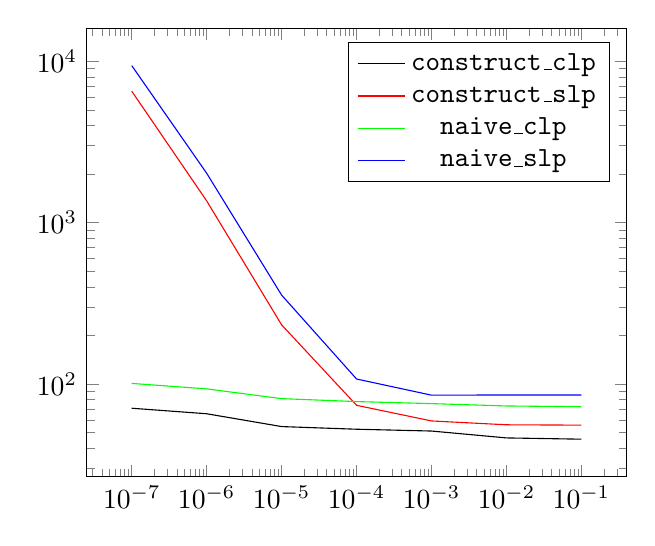
\begin{tikzpicture}
    \begin{loglogaxis}[
        legend pos=north east]

        \addplot[black] plot coordinates {
(0.1,       45.51)
(0.01,      46.34)
(0.001,     51.12)
(0.0001,    52.46)
(0.00001,   54.48)
(0.000001,  65.42)
(0.0000001, 70.78)
        };

        \addplot[red] plot coordinates {
(0.1,       55.61)
(0.01,      55.89)
(0.001,     59.04)
(0.0001,    73.79)
(0.00001,   232.53)
(0.000001,  1363.46)
(0.0000001, 6522.91)
        };

        \addplot[green] plot coordinates {
(0.1,       72.32)
(0.01,      73.11)
(0.001,     75.60)
(0.0001,    77.83)
(0.00001,   81.16)
(0.000001,  93.29)
(0.0000001, 100.85)
        };

        \addplot[blue] plot coordinates {
(0.1,       85.51)
(0.01,      85.51)
(0.001,     85.28)
(0.0001,    107.39)
(0.00001,   355.47)
(0.000001,  2022.25)
(0.0000001, 9395.92)
        };

        \legend{\texttt{construct\_clp}, \texttt{construct\_slp}, \texttt{naive\_clp}, \texttt{naive\_slp}}
    \end{loglogaxis}
\end{tikzpicture}

    \caption{Seconds used to solve \textit{small} and $s(2, 238)$ of its
             subinstances with different tolerances.
             The x-axis represents the tolerance $\epsilon$.
             The y-axis represents the number of seconds used.}
    \label{fig:smalltolerance}
\end{figure}
We can measure the number of Slp iterations required to solve a given problem
given some tolerance. By solving randomly generated problems where $n = 50$,
with Slp, we note the average number of iterations among ten solved
problems. Table \ref{table:expiters} shows the results from this, and we see
that the average number of iterations increases rapidly as the tolerance
becomes smaller than $10^{-4}$. This fits our prediction about why
\texttt{cSlp} and \texttt{nSlp} becomes much slower at lower tolerances.

\begin{table}[ht!]
\centering
\caption{Average number of iterations used by Slp with different tolerances,
         to solve ten randomly generated instances.}
\label{table:expiters}
\begin{tabular}{rrrrr}
$\epsilon$ & Iterations \\ \hline
$10^{-1}$  & 1 \\
$10^{-2}$  & 1.8 \\
$10^{-3}$  & 2.2 \\
$10^{-4}$  & 3.5 \\
$10^{-5}$  & 8.6 \\
$10^{-6}$  & 23.7 \\
$10^{-7}$  & 90.1 \\
$10^{-8}$  & 223.5 \\
$10^{-9}$  & 752.6
\end{tabular}
\end{table}

\subsubsection{Experiment 2}
In this experiment we let $\epsilon = 10^{-4}$, so that the implementations
of Slp may keep up. Table \ref{table:eps4instances} shows the results from
this experiment.
Unfortunately, we see that even with a high tolerance, Slp can not keep up as
$n$ increases.

\begin{table}
\centering
\caption{Results from Experiment 2.}
\label{table:eps4instances}
\begin{tabular}{crrr}
\textrm{Implementation} & \textit{small} & \textit{large} & \textit{vlarge} \\ \hline
\texttt{cClp}           & 0.52           & 9.55           & 76.18 \\
\texttt{cSlp}           & 0.71           & 32.88          & 585.60 \\
\texttt{nClp}           & 0.65           & 11.68          & 157.53 \\
\texttt{nSlp}           & 0.89           & 39.87          & 1173.74
\end{tabular}
\end{table}

\subsubsection{Experiment 3}
Table \ref{table:expfour} shows an excerpt of the test results.
A table with results for all $n=100,200,\ldots,2000$ can found in Appendix
\ref{app:exp1}.
We see that, as the problem size grows, the \texttt{cClp}
implementation becomes faster and faster in comparison with
\texttt{nClp}.
This is due to the fact that we save more time for each problem we do
\emph{not} need to solve, as $n$ becomes larger, simply because larger problems
take more time to solve.
There are also more subinstances as
$n$ grows, making room for more subinstances that we might not have to solve.

\begin{table}[ht!]
    \centering
    \caption{An excerpt of test results from Experiment 3.
             The values in the \texttt{cClp} and \texttt{nClp} columns are the
             average running times in seconds for solving instances with
             $s(1, n)$ subinstances, ten times.
             The rightmost column represents how much faster, in percent,
             \texttt{cClp} is compared with \texttt{nClp}.}
    \label{table:expfour}
\begin{tabular}{rrrc}
    $n$ & \texttt{cClp}  & \texttt{nClp}  & Faster \\ \hline
    500 & 4.9   & 5.9   & 16.9\% \\
   1000 & 42.1  & 53.0  & 20.6\% \\
   1500 & 181.5 & 234.5 & 22.6\% \\
   2000 & 547.1 & 710.2 & 23.0\%
\end{tabular}
\end{table}

\subsubsection{Experiment 4}
Table \ref{table:exptwo} shows the test results from this experiment. We see
that, as $b$ increases, the \texttt{cClp} implementation becomes
faster and faster in comparison with \texttt{nClp}.
This is due to the fact that as the tree grows in size, the chance that
an unsolved subinstance is distinct, decreases. In fact, looking at the
rightmost column in Table \ref{table:exptwo}, we can calculate the percentage
of distinct solutions as $b$ increases.
There are $74.3\%, 58.3\%, 45.4\%, 32.8\%$ and $24.2\%$ distinct solutions for
$b$ equal to $1,2,3,4$ and $5$, respectively. This helps us clarify the reason
why \texttt{cClp} becomes faster and faster in comparison with \texttt{nClp}.
\begin{table}[ht!]
\centering
\caption{Results from experiment 4.
         The values in the \texttt{cClp} and \texttt{nClp} columns are the
         average running times in seconds for solving instances where $n = 50$,
         with $s(b, 50)$ subinstances, ten times.
         The Faster column represents how much faster, in percent,
         \texttt{cClp} is compared with \texttt{nClp}.
         The Skipped column represents how many subinstances we could skip
         solving because its solution was found in the tree.
         }
\begin{tabular}{rrrcr}
      $b$ & \texttt{cClp} & \texttt{nClp} & Faster & Skipped\\ \hline
       1  & 0.03 & 0.04 & 25.0\% & 13.6 \\
       2  & 0.64 & 0.94 & 31.9\% & 531.7 \\
       3  & 7.06 & 15.90 & 55.6\% & 11391.3 \\
       4  & 77.59 & 188.83 & 58.9\% & 168913.5 \\
       5  & 586.54 & 1758.23 & 66.6\% & 1795250.7 \\
\end{tabular}
\label{table:exptwo}
\end{table}

Figure \ref{fig:constructincb} shows a plot of the number of seconds used to
solve, on average, one subinstance, as $b$ increases.
We see that as $b$ increases, the number of
seconds to solve one subinstance decreases with \texttt{cClp},
but with \texttt{nClp}, it does not change much. This behavior is very
much expected, especially considering our earlier assessment in this
experiment.

\begin{figure}[ht!]
    \centering
    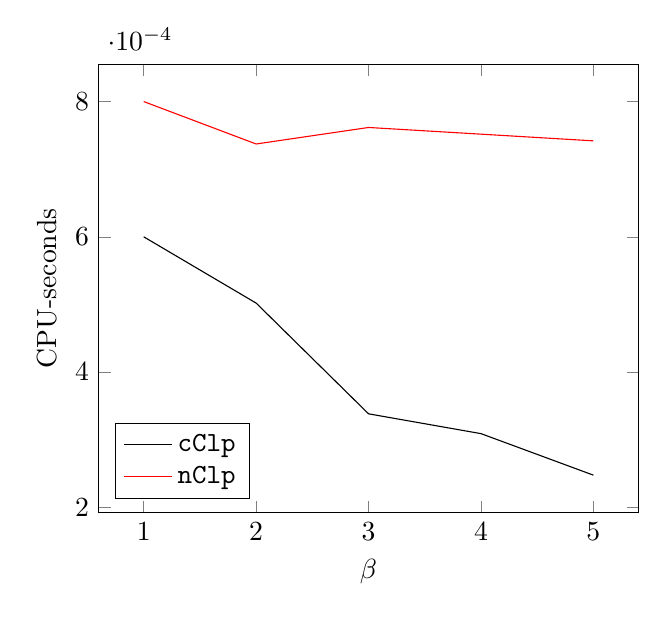
\begin{tikzpicture}
    \begin{axis}[
        xlabel=$\beta$,
        ylabel=CPU-seconds,
        legend pos=south west]

        \addplot[black] plot coordinates {
(1, 0.0006)
(2, 0.000501961)
(3, 0.000338204)
(4, 0.000308908)
(5, 0.000247492)
        };

        \addplot[red] plot coordinates {
(1, 0.0008)
(2, 0.000737255)
(3, 0.000761677)
(4, 0.000751787)
(5, 0.00074189)
        };

        \legend{\texttt{cClp}, \texttt{nClp}}
    \end{axis}
\end{tikzpicture}

    \caption{Seconds used, on average, to solve one subinstance, as $b$
             increases.
             The x-axis represents $b$.
             The y-axis represents the number of seconds used, on average,
             to solve one subinstance.}
    \label{fig:constructincb}
\end{figure}

%\subsubsection{Experiment 5}
\begin{table}[ht!]
\centering
\caption{Ignore this table at the moment. Unfinished possible experiment.}
\begin{tabular}{rrrr}
    $b$ & \texttt{cClp} & \texttt{cSlp} & Skipped \\ \hline
     1  & 0.01          &               & 6.2 \\
     2  & 0.08          &               & 131.5 \\
     3  & 0.48          &               & 1237.3 \\
     4  & 2.16          &               & 9579.5 \\
     5  & 6.23          &               & 50825.9 \\
     6  & 18.52         &               & 201651.9 \\
     7  & 70.16         &               & 567071.6 \\
     8  & 202.11        &               & 1462074.6 \\
     9  & 379.84        &               & 3351206.6 \\
     10 & 807.85        &               & 6468142.0
\end{tabular}
\end{table}
